\chapter{Cluster algebras of surface type}
Before we begin, we define what we mean by \emph{surface}, or of \emph{ surface type};
\begin{definition}
A \emph{surface} $(S,M)$ is a connected oriented Riemann surface $S$ with (possibly empty) boundary $\partial S$; together with a finite collection $M \subset S$ of \emph{marked points}; with the only condition that each boundary component $\mathbf{must}$ contain at least one marked point.
\end{definition}
\begin{figure}[H]
    \centering
    

\tikzset{every picture/.style={line width=0.75pt}} %set default line width to 0.75pt        

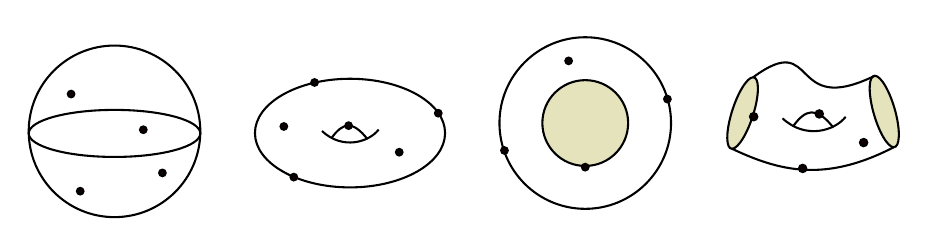
\begin{tikzpicture}[x=0.75pt,y=0.75pt,yscale=-1,xscale=1]
%uncomment if require: \path (0,471); %set diagram left start at 0, and has height of 471

%Shape: Ellipse [id:dp5936664030318399] 
\draw   (99,83.33) .. controls (99,77.07) and (117.51,72) .. (140.33,72) .. controls (163.16,72) and (181.67,77.07) .. (181.67,83.33) .. controls (181.67,89.59) and (163.16,94.67) .. (140.33,94.67) .. controls (117.51,94.67) and (99,89.59) .. (99,83.33) -- cycle ;
%Shape: Circle [id:dp886964729900558] 
\draw   (99,82.33) .. controls (99,59.51) and (117.51,41) .. (140.33,41) .. controls (163.16,41) and (181.67,59.51) .. (181.67,82.33) .. controls (181.67,105.16) and (163.16,123.67) .. (140.33,123.67) .. controls (117.51,123.67) and (99,105.16) .. (99,82.33) -- cycle ;
%Shape: Circle [id:dp9505094746069663] 
\draw   (325.8,78.33) .. controls (325.8,55.51) and (344.31,37) .. (367.13,37) .. controls (389.96,37) and (408.47,55.51) .. (408.47,78.33) .. controls (408.47,101.16) and (389.96,119.67) .. (367.13,119.67) .. controls (344.31,119.67) and (325.8,101.16) .. (325.8,78.33) -- cycle ;
%Shape: Circle [id:dp0899912035587026] 
\draw  [fill={rgb, 255:red, 15; green, 1; blue, 1 }  ,fill opacity=1 ] (117.83,64.35) .. controls (117.83,63.47) and (118.55,62.77) .. (119.43,62.78) .. controls (120.31,62.78) and (121.01,63.5) .. (121,64.38) .. controls (120.99,65.26) and (120.27,65.96) .. (119.4,65.95) .. controls (118.52,65.94) and (117.82,65.23) .. (117.83,64.35) -- cycle ;
%Shape: Circle [id:dp6344129113519207] 
\draw  [fill={rgb, 255:red, 15; green, 1; blue, 1 }  ,fill opacity=1 ] (152.63,81.55) .. controls (152.63,80.67) and (153.35,79.97) .. (154.23,79.98) .. controls (155.11,79.98) and (155.81,80.7) .. (155.8,81.58) .. controls (155.79,82.46) and (155.07,83.16) .. (154.2,83.15) .. controls (153.32,83.14) and (152.62,82.43) .. (152.63,81.55) -- cycle ;
%Shape: Circle [id:dp4511676376300491] 
\draw  [fill={rgb, 255:red, 15; green, 1; blue, 1 }  ,fill opacity=1 ] (122.23,111.15) .. controls (122.23,110.27) and (122.95,109.57) .. (123.83,109.58) .. controls (124.71,109.58) and (125.41,110.3) .. (125.4,111.18) .. controls (125.39,112.06) and (124.67,112.76) .. (123.8,112.75) .. controls (122.92,112.74) and (122.22,112.03) .. (122.23,111.15) -- cycle ;
%Shape: Circle [id:dp4148375320769103] 
\draw  [fill={rgb, 255:red, 15; green, 1; blue, 1 }  ,fill opacity=1 ] (161.83,102.35) .. controls (161.83,101.47) and (162.55,100.77) .. (163.43,100.78) .. controls (164.31,100.78) and (165.01,101.5) .. (165,102.38) .. controls (164.99,103.26) and (164.27,103.96) .. (163.4,103.95) .. controls (162.52,103.94) and (161.82,103.23) .. (161.83,102.35) -- cycle ;
%Shape: Circle [id:dp13358398817698114] 
\draw  [fill={rgb, 255:red, 228; green, 227; blue, 188 }  ,fill opacity=1 ] (346.47,78.33) .. controls (346.47,66.92) and (355.72,57.67) .. (367.13,57.67) .. controls (378.55,57.67) and (387.8,66.92) .. (387.8,78.33) .. controls (387.8,89.75) and (378.55,99) .. (367.13,99) .. controls (355.72,99) and (346.47,89.75) .. (346.47,78.33) -- cycle ;
%Shape: Circle [id:dp8855500282436761] 
\draw  [fill={rgb, 255:red, 15; green, 1; blue, 1 }  ,fill opacity=1 ] (326.63,91.55) .. controls (326.63,90.67) and (327.35,89.97) .. (328.23,89.98) .. controls (329.11,89.98) and (329.81,90.7) .. (329.8,91.58) .. controls (329.79,92.46) and (329.07,93.16) .. (328.2,93.15) .. controls (327.32,93.14) and (326.62,92.43) .. (326.63,91.55) -- cycle ;
%Shape: Circle [id:dp9212146321694251] 
\draw  [fill={rgb, 255:red, 15; green, 1; blue, 1 }  ,fill opacity=1 ] (365.53,99.57) .. controls (365.54,98.7) and (366.26,97.99) .. (367.13,98) .. controls (368.01,98.01) and (368.71,98.73) .. (368.71,99.6) .. controls (368.7,100.48) and (367.98,101.18) .. (367.1,101.18) .. controls (366.23,101.17) and (365.52,100.45) .. (365.53,99.57) -- cycle ;
%Shape: Circle [id:dp9296470673413565] 
\draw  [fill={rgb, 255:red, 15; green, 1; blue, 1 }  ,fill opacity=1 ] (405.13,66.77) .. controls (405.14,65.9) and (405.86,65.19) .. (406.73,65.2) .. controls (407.61,65.21) and (408.31,65.93) .. (408.31,66.8) .. controls (408.3,67.68) and (407.58,68.38) .. (406.7,68.38) .. controls (405.83,68.37) and (405.12,67.65) .. (405.13,66.77) -- cycle ;
%Shape: Circle [id:dp9075391788904883] 
\draw  [fill={rgb, 255:red, 15; green, 1; blue, 1 }  ,fill opacity=1 ] (357.53,48.37) .. controls (357.54,47.5) and (358.26,46.79) .. (359.13,46.8) .. controls (360.01,46.81) and (360.71,47.53) .. (360.71,48.4) .. controls (360.7,49.28) and (359.98,49.98) .. (359.1,49.98) .. controls (358.23,49.97) and (357.52,49.25) .. (357.53,48.37) -- cycle ;
%Shape: Ellipse [id:dp4018320458815504] 
\draw   (208,83.17) .. controls (208,68.72) and (228.51,57) .. (253.8,57) .. controls (279.09,57) and (299.6,68.72) .. (299.6,83.17) .. controls (299.6,97.63) and (279.09,109.34) .. (253.8,109.34) .. controls (228.51,109.34) and (208,97.63) .. (208,83.17) -- cycle ;
%Curve Lines [id:da03186435929475773] 
\draw    (240.27,82.17) .. controls (250.27,91.5) and (262.93,87.5) .. (267.6,81.5) ;
%Curve Lines [id:da7981103996078125] 
\draw    (244.93,85.5) .. controls (250.27,78.17) and (254.93,76.83) .. (262.27,86.17) ;
%Curve Lines [id:da8812010320833625] 
\draw    (462.18,76.07) .. controls (473.31,86.46) and (487.41,82.01) .. (492.6,75.33) ;
%Curve Lines [id:da6506246829588368] 
\draw    (467.37,79.78) .. controls (473.31,71.62) and (478.5,70.14) .. (486.66,80.52) ;
%Shape: Ellipse [id:dp9250644288260443] 
\draw  [fill={rgb, 255:red, 228; green, 227; blue, 188 }  ,fill opacity=1 ] (437.59,73.51) .. controls (440.4,64) and (445.08,56.29) .. (448.03,56.29) .. controls (450.99,56.29) and (451.11,64) .. (448.3,73.51) .. controls (445.49,83.02) and (440.81,90.74) .. (437.86,90.74) .. controls (434.9,90.74) and (434.78,83.02) .. (437.59,73.51) -- cycle ;
%Shape: Ellipse [id:dp5372444143214322] 
\draw  [fill={rgb, 255:red, 228; green, 227; blue, 188 }  ,fill opacity=1 ] (505.85,72.77) .. controls (503.34,63.26) and (503.69,55.55) .. (506.65,55.55) .. controls (509.61,55.55) and (514.04,63.26) .. (516.56,72.77) .. controls (519.07,82.28) and (518.71,89.99) .. (515.76,89.99) .. controls (512.8,89.99) and (508.37,82.28) .. (505.85,72.77) -- cycle ;
%Curve Lines [id:da07938845410908513] 
\draw    (437.86,90.74) .. controls (460.62,101.45) and (482.44,107.23) .. (515.76,89.99) ;
%Curve Lines [id:da039009680495956545] 
\draw    (448.03,56.29) .. controls (479.76,32.89) and (464.63,76.07) .. (506.65,55.55) ;
%Shape: Circle [id:dp3402244483606086] 
\draw  [fill={rgb, 255:red, 15; green, 1; blue, 1 }  ,fill opacity=1 ] (251.53,79.57) .. controls (251.54,78.7) and (252.26,77.99) .. (253.13,78) .. controls (254.01,78.01) and (254.71,78.73) .. (254.71,79.6) .. controls (254.7,80.48) and (253.98,81.18) .. (253.1,81.18) .. controls (252.23,81.17) and (251.52,80.45) .. (251.53,79.57) -- cycle ;
%Shape: Circle [id:dp1515362552946773] 
\draw  [fill={rgb, 255:red, 15; green, 1; blue, 1 }  ,fill opacity=1 ] (225.13,104.37) .. controls (225.14,103.5) and (225.86,102.79) .. (226.73,102.8) .. controls (227.61,102.81) and (228.31,103.53) .. (228.31,104.4) .. controls (228.3,105.28) and (227.58,105.98) .. (226.7,105.98) .. controls (225.83,105.97) and (225.12,105.25) .. (225.13,104.37) -- cycle ;
%Shape: Circle [id:dp540351092308096] 
\draw  [fill={rgb, 255:red, 15; green, 1; blue, 1 }  ,fill opacity=1 ] (275.93,92.37) .. controls (275.94,91.5) and (276.66,90.79) .. (277.53,90.8) .. controls (278.41,90.81) and (279.11,91.53) .. (279.11,92.4) .. controls (279.1,93.28) and (278.38,93.98) .. (277.5,93.98) .. controls (276.63,93.97) and (275.92,93.25) .. (275.93,92.37) -- cycle ;
%Shape: Circle [id:dp056198737530079645] 
\draw  [fill={rgb, 255:red, 15; green, 1; blue, 1 }  ,fill opacity=1 ] (235.13,58.77) .. controls (235.14,57.9) and (235.86,57.19) .. (236.73,57.2) .. controls (237.61,57.21) and (238.31,57.93) .. (238.31,58.8) .. controls (238.3,59.68) and (237.58,60.38) .. (236.7,60.38) .. controls (235.83,60.37) and (235.12,59.65) .. (235.13,58.77) -- cycle ;
%Shape: Circle [id:dp4449482163456263] 
\draw  [fill={rgb, 255:red, 15; green, 1; blue, 1 }  ,fill opacity=1 ] (294.73,73.57) .. controls (294.74,72.7) and (295.46,71.99) .. (296.33,72) .. controls (297.21,72.01) and (297.91,72.73) .. (297.91,73.6) .. controls (297.9,74.48) and (297.18,75.18) .. (296.3,75.18) .. controls (295.43,75.17) and (294.72,74.45) .. (294.73,73.57) -- cycle ;
%Shape: Circle [id:dp5622367823369225] 
\draw  [fill={rgb, 255:red, 15; green, 1; blue, 1 }  ,fill opacity=1 ] (220.33,79.97) .. controls (220.34,79.1) and (221.06,78.39) .. (221.93,78.4) .. controls (222.81,78.41) and (223.51,79.13) .. (223.51,80) .. controls (223.5,80.88) and (222.78,81.58) .. (221.9,81.58) .. controls (221.03,81.57) and (220.32,80.85) .. (220.33,79.97) -- cycle ;
%Shape: Ellipse [id:dp8536461228034546] 
\draw  [fill={rgb, 255:red, 15; green, 1; blue, 1 }  ,fill opacity=1 ] (446.51,75.26) .. controls (446.52,74.29) and (447.32,73.5) .. (448.3,73.51) .. controls (449.27,73.52) and (450.06,74.32) .. (450.05,75.3) .. controls (450.04,76.27) and (449.24,77.05) .. (448.26,77.05) .. controls (447.29,77.04) and (446.5,76.24) .. (446.51,75.26) -- cycle ;
%Shape: Ellipse [id:dp15602120118848628] 
\draw  [fill={rgb, 255:red, 15; green, 1; blue, 1 }  ,fill opacity=1 ] (470.11,100.19) .. controls (470.12,99.21) and (470.92,98.43) .. (471.89,98.44) .. controls (472.87,98.45) and (473.65,99.25) .. (473.64,100.22) .. controls (473.63,101.2) and (472.83,101.98) .. (471.86,101.97) .. controls (470.88,101.96) and (470.1,101.17) .. (470.11,100.19) -- cycle ;
%Shape: Ellipse [id:dp7286045659331059] 
\draw  [fill={rgb, 255:red, 15; green, 1; blue, 1 }  ,fill opacity=1 ] (478.12,73.93) .. controls (478.13,72.95) and (478.93,72.17) .. (479.9,72.18) .. controls (480.88,72.19) and (481.66,72.98) .. (481.65,73.96) .. controls (481.64,74.94) and (480.85,75.72) .. (479.87,75.71) .. controls (478.89,75.7) and (478.11,74.9) .. (478.12,73.93) -- cycle ;
%Shape: Ellipse [id:dp9636443945093016] 
\draw  [fill={rgb, 255:red, 15; green, 1; blue, 1 }  ,fill opacity=1 ] (499.49,87.73) .. controls (499.5,86.75) and (500.3,85.97) .. (501.27,85.98) .. controls (502.25,85.99) and (503.03,86.78) .. (503.02,87.76) .. controls (503.01,88.74) and (502.21,89.52) .. (501.24,89.51) .. controls (500.26,89.5) and (499.48,88.7) .. (499.49,87.73) -- cycle ;




\end{tikzpicture}

    \caption{Examples of marked surfaces, with 0, 0, 1, and 2 boundary components, respectively.}
\end{figure}
Any marked point $p \in M$ such that $p \notin \partial S$ is referred to as a \emph{puncture}.
Once we have a surface, we define additional structures.\begin{definition}(\emph{Ordinary arcs}) 
    An \emph{arc} $\gamma$ in $(S,M)$ is a curve in $S$, considered up to isotopy, such that;
    \begin{itemize}
        \item Its endpoints are in $M$,
        \item It does not intersect itself, except for possibly having overlapping endpoints,
        \item Besides its endpoints, $\gamma$ is disjoint from $M$,
        \item $\gamma$ does not cut out an unpunctured monogon or bigon.
    \end{itemize}
\end{definition}
For the sake of labeling, an arc that starts and ends in the same points is called a \emph{loop}.
Moreover, suppose we have two arcs $\gamma, \tilde{\gamma}$ on a surface $S$, then we define $e(\gamma, \tilde{\gamma})$ to be the number of intersections between the two arcs when considering all possible isotopy\footnote{An \emph{isotopy} is a homotopy $h: [0,1]\times X \to Y$ such that for each $t \in [0,1]$, $h(t,\bullet)$ is a homeomorphism.} equivalent arcs for both. If $e(\gamma,\tilde{\gamma}) = 0$, then we say that the arcs $\gamma$ and $\tilde{\gamma}$ are compatible. If a maximal triangulation $T$ consists entirely of pairwise compatible arcs, then it is called an \emph{ideal triangulation}, which each triangular region called an \emph{ideal triangle}.
\begin{figure}[H]
    \centering
    

\tikzset{every picture/.style={line width=0.75pt}} %set default line width to 0.75pt        

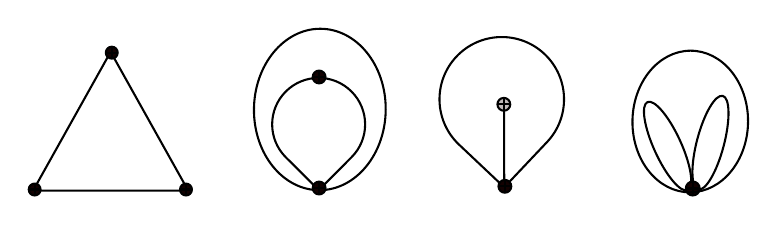
\begin{tikzpicture}[x=0.75pt,y=0.75pt,yscale=-1,xscale=1]
%uncomment if require: \path (0,471); %set diagram left start at 0, and has height of 471

%Shape: Triangle [id:dp9282044160141008] 
\draw   (150.39,93.31) -- (187.77,160.18) -- (113.01,160.18) -- cycle ;
\draw  [fill={rgb, 255:red, 19; green, 1; blue, 1 }  ,fill opacity=1 ] (110.92,159.64) .. controls (110.92,158.05) and (112.2,156.77) .. (113.78,156.77) .. controls (115.36,156.77) and (116.64,158.05) .. (116.64,159.64) .. controls (116.64,161.22) and (115.36,162.5) .. (113.78,162.5) .. controls (112.2,162.5) and (110.92,161.22) .. (110.92,159.64) -- cycle ; \draw   (110.92,159.64) -- (116.64,159.64) ; \draw   (113.78,156.77) -- (113.78,162.5) ;
\draw  [fill={rgb, 255:red, 19; green, 1; blue, 1 }  ,fill opacity=1 ] (183.82,159.64) .. controls (183.82,158.05) and (185.1,156.77) .. (186.69,156.77) .. controls (188.27,156.77) and (189.55,158.05) .. (189.55,159.64) .. controls (189.55,161.22) and (188.27,162.5) .. (186.69,162.5) .. controls (185.1,162.5) and (183.82,161.22) .. (183.82,159.64) -- cycle ; \draw   (183.82,159.64) -- (189.55,159.64) ; \draw   (186.69,156.77) -- (186.69,162.5) ;
\draw  [fill={rgb, 255:red, 19; green, 1; blue, 1 }  ,fill opacity=1 ] (148.07,93.7) .. controls (148.07,92.12) and (149.35,90.83) .. (150.93,90.83) .. controls (152.51,90.83) and (153.79,92.12) .. (153.79,93.7) .. controls (153.79,95.28) and (152.51,96.56) .. (150.93,96.56) .. controls (149.35,96.56) and (148.07,95.28) .. (148.07,93.7) -- cycle ; \draw   (148.07,93.7) -- (153.79,93.7) ; \draw   (150.93,90.83) -- (150.93,96.56) ;
%Shape: Tear Drop [id:dp6032198370858309] 
\draw   (234.8,144.12) .. controls (234.8,144.12) and (234.8,144.12) .. (234.8,144.12) .. controls (226.04,135.39) and (226.01,121.21) .. (234.74,112.45) .. controls (243.47,103.69) and (257.65,103.66) .. (266.41,112.39) .. controls (275.17,121.12) and (275.2,135.3) .. (266.47,144.06) .. controls (255.94,154.63) and (250.66,159.93) .. (250.66,159.93) .. controls (250.66,159.93) and (245.38,154.66) .. (234.8,144.12) -- cycle ;
%Shape: Ellipse [id:dp3071299319516321] 
\draw   (251.34,82.18) .. controls (268.87,82.16) and (283,99.54) .. (282.92,121.02) .. controls (282.83,142.49) and (268.55,159.92) .. (251.03,159.95) .. controls (233.5,159.98) and (219.36,142.59) .. (219.44,121.12) .. controls (219.53,99.64) and (233.81,82.21) .. (251.34,82.18) -- cycle ;
\draw  [fill={rgb, 255:red, 19; green, 1; blue, 1 }  ,fill opacity=1 ] (247.75,158.92) .. controls (247.75,157.21) and (249.13,155.83) .. (250.83,155.83) .. controls (252.54,155.83) and (253.92,157.21) .. (253.92,158.92) .. controls (253.92,160.62) and (252.54,162) .. (250.83,162) .. controls (249.13,162) and (247.75,160.62) .. (247.75,158.92) -- cycle ; \draw   (247.75,158.92) -- (253.92,158.92) ; \draw   (250.83,155.83) -- (250.83,162) ;
\draw  [fill={rgb, 255:red, 19; green, 1; blue, 1 }  ,fill opacity=1 ] (247.75,105.42) .. controls (247.75,103.71) and (249.13,102.33) .. (250.83,102.33) .. controls (252.54,102.33) and (253.92,103.71) .. (253.92,105.42) .. controls (253.92,107.12) and (252.54,108.5) .. (250.83,108.5) .. controls (249.13,108.5) and (247.75,107.12) .. (247.75,105.42) -- cycle ; \draw   (247.75,105.42) -- (253.92,105.42) ; \draw   (250.83,102.33) -- (250.83,108.5) ;
%Shape: Tear Drop [id:dp6386482616728619] 
\draw   (318.22,137.97) .. controls (318.22,137.97) and (318.22,137.97) .. (318.22,137.97) .. controls (318.22,137.97) and (318.22,137.97) .. (318.22,137.97) .. controls (306.18,126.59) and (305.65,107.6) .. (317.03,95.56) .. controls (328.41,83.52) and (347.4,82.98) .. (359.44,94.37) .. controls (371.48,105.75) and (372.02,124.74) .. (360.63,136.78) .. controls (360.63,136.78) and (360.63,136.78) .. (360.63,136.78) .. controls (346.89,151.3) and (340.03,158.57) .. (340.03,158.58) .. controls (340.03,158.57) and (332.76,151.7) .. (318.22,137.97) -- cycle ;
%Straight Lines [id:da4842260407951211] 
\draw    (340.03,158.58) -- (339.92,119.08) ;
\draw  [fill={rgb, 255:red, 19; green, 1; blue, 1 }  ,fill opacity=1 ] (337.25,158.08) .. controls (337.25,156.38) and (338.63,155) .. (340.33,155) .. controls (342.04,155) and (343.42,156.38) .. (343.42,158.08) .. controls (343.42,159.79) and (342.04,161.17) .. (340.33,161.17) .. controls (338.63,161.17) and (337.25,159.79) .. (337.25,158.08) -- cycle ; \draw   (337.25,158.08) -- (343.42,158.08) ; \draw   (340.33,155) -- (340.33,161.17) ;
\draw  [fill={rgb, 255:red, 192; green, 185; blue, 185 }  ,fill opacity=1 ] (336.75,118.58) .. controls (336.75,116.88) and (338.13,115.5) .. (339.83,115.5) .. controls (341.54,115.5) and (342.92,116.88) .. (342.92,118.58) .. controls (342.92,120.29) and (341.54,121.67) .. (339.83,121.67) .. controls (338.13,121.67) and (336.75,120.29) .. (336.75,118.58) -- cycle ; \draw   (336.75,118.58) -- (342.92,118.58) ; \draw   (339.83,115.5) -- (339.83,121.67) ;
%Shape: Ellipse [id:dp6950674907452231] 
\draw   (409.03,117.51) .. controls (412.32,116) and (419.33,124.27) .. (424.69,135.98) .. controls (430.04,147.68) and (431.71,158.39) .. (428.42,159.9) .. controls (425.13,161.41) and (418.12,153.14) .. (412.76,141.43) .. controls (407.41,129.73) and (405.74,119.01) .. (409.03,117.51) -- cycle ;
%Shape: Ellipse [id:dp09560336913224654] 
\draw   (445.33,114.53) .. controls (448.83,115.46) and (449.01,126.3) .. (445.72,138.74) .. controls (442.44,151.19) and (436.94,160.54) .. (433.44,159.61) .. controls (429.94,158.69) and (429.76,147.85) .. (433.04,135.4) .. controls (436.33,122.95) and (441.82,113.61) .. (445.33,114.53) -- cycle ;
\draw  [fill={rgb, 255:red, 19; green, 1; blue, 1 }  ,fill opacity=1 ] (427.51,159.15) .. controls (427.51,157.3) and (429.01,155.79) .. (430.86,155.79) .. controls (432.71,155.79) and (434.21,157.3) .. (434.21,159.15) .. controls (434.21,161) and (432.71,162.5) .. (430.86,162.5) .. controls (429.01,162.5) and (427.51,161) .. (427.51,159.15) -- cycle ; \draw   (427.51,159.15) -- (434.21,159.15) ; \draw   (430.86,155.79) -- (430.86,162.5) ;
%Shape: Ellipse [id:dp675764835830011] 
\draw   (429.78,92.75) .. controls (445.16,92.73) and (457.57,107.98) .. (457.49,126.83) .. controls (457.42,145.67) and (444.89,160.96) .. (429.51,160.99) .. controls (414.13,161.01) and (401.72,145.76) .. (401.8,126.91) .. controls (401.87,108.07) and (414.4,92.77) .. (429.78,92.75) -- cycle ;




\end{tikzpicture}

    \caption{Ordinary triangle, two-vertex triangle, self-folded triangle and one-vertex triangle.}
\end{figure}
In the figure above we see the four possible types of ideal triangles in a possible ideal triangulation. In this paper we will focus mostly on the first (and perhaps the fourth one too) as the other two require a marked point that is not on any boundary component; which we will often not consider for the sake of length and clarity. 
\begin{theorem}{\normalfont \cite{Sch}}
The number of arcs in an ideal triangulation is exactly
\begin{equation*}
    n = 6g + 3b + 3p + c - 6;
\end{equation*}
where $g$ is the genus of $S$, $b$ is the number of boundary components, $p$ is the number of punctures and $c = |M|-p$ is the number of marked points on $\partial S$.
\end{theorem}
\begin{remark}
Note that each ideal triangulation is connected to all other possible triangulations by a series of \emph{flips}; that is, replacing an arc $\gamma$ by another arc $\Tilde{\gamma}$, so to obtain our new triangulation $\Tilde{T} = (T\backslash\{\gamma\}) \cup \{\Tilde{\gamma}\}$, in the following way; 
\begin{figure}[H]
    \centering
    

\tikzset{every picture/.style={line width=0.75pt}} %set default line width to 0.75pt        

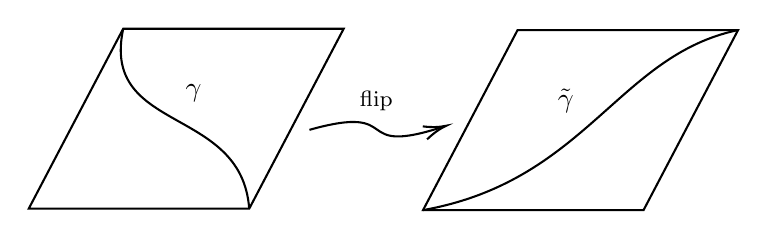
\begin{tikzpicture}[x=0.75pt,y=0.75pt,yscale=-1,xscale=1]
%uncomment if require: \path (0,342); %set diagram left start at 0, and has height of 342

%Shape: Parallelogram [id:dp9440132437357889] 
\draw   (106.2,82.67) -- (212.43,82.67) -- (166.9,169.39) -- (60.67,169.39) -- cycle ;
%Shape: Parallelogram [id:dp4450674539847944] 
\draw   (296.2,83.33) -- (402.43,83.33) -- (356.9,170.06) -- (250.67,170.06) -- cycle ;
%Curve Lines [id:da015686636387745367] 
\draw    (106.2,82.67) .. controls (95.28,133.39) and (163.28,119.39) .. (166.9,169.39) ;
%Curve Lines [id:da5146201674257586] 
\draw    (250.67,170.06) .. controls (329.28,156.06) and (344.61,95.39) .. (402.43,83.33) ;
%Curve Lines [id:da8815901966148098] 
\draw    (195.94,131.39) .. controls (242.8,118.19) and (214.52,144.85) .. (260.53,129.86) ;
\draw [shift={(261.94,129.39)}, rotate = 161.57] [color={rgb, 255:red, 0; green, 0; blue, 0 }  ][line width=0.75]    (10.93,-3.29) .. controls (6.95,-1.4) and (3.31,-0.3) .. (0,0) .. controls (3.31,0.3) and (6.95,1.4) .. (10.93,3.29)   ;

% Text Node
\draw (134.78,108.07) node [anchor=north west][inner sep=0.75pt]    {$\gamma $};
% Text Node
\draw (314.11,110.07) node [anchor=north west][inner sep=0.75pt]    {$\tilde{\gamma }$};
% Text Node
\draw (218.78,111.33) node [anchor=north west][inner sep=0.75pt]   [align=left] {{\footnotesize flip}};


\end{tikzpicture}

    \caption{Example of flip at arc $\gamma$.}
\end{figure}
\end{remark}


\section{Cluster algebras from surfaces}
Now that we outlined the necessary definition, we will define the cluster algebra associated to a surface.
Let $T = \{\tau_1, \dots, \tau_n\}$ be an ideal trangulation of a surface $(S,M)$, and $\mathcal{Q}_T$ a cluster quiver defined as follows.
The vertices of $\mathcal{Q}_T$ are in bijection with the arcs of $T$; i.e. $\tau_i \mapsto i$. The arrows of $\mathcal{Q}_T$ are determined in the following way; for any triangle $\Delta$ in $T$, we draw an arrow $i \to j$ if $\tau_i$ and $\tau_j$ are sides of $\Delta$ with $\tau_j$ following $\tau_i$ in the clockwise order.
\begin{figure}[H]
    \centering
    

\tikzset{every picture/.style={line width=0.75pt}} %set default line width to 0.75pt        

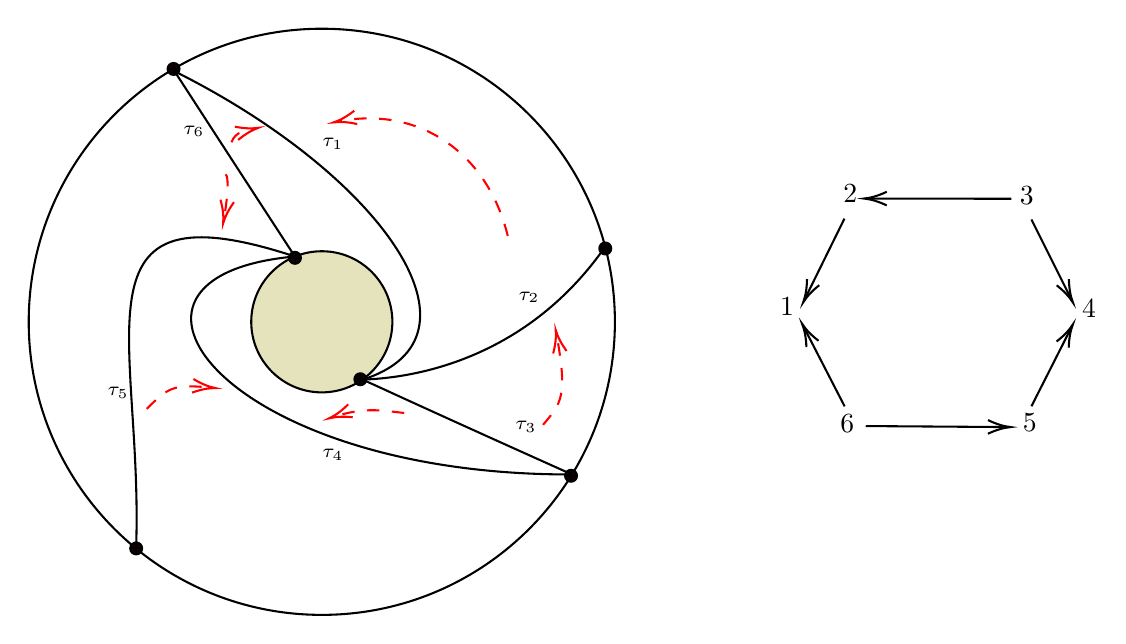
\begin{tikzpicture}[x=0.75pt,y=0.75pt,yscale=-1,xscale=1]
%uncomment if require: \path (0,458); %set diagram left start at 0, and has height of 458

%Shape: Circle [id:dp011167431945667827] 
\draw   (11,248.38) .. controls (11,170.39) and (74.22,107.17) .. (152.21,107.17) .. controls (230.2,107.17) and (293.42,170.39) .. (293.42,248.38) .. controls (293.42,326.36) and (230.2,389.58) .. (152.21,389.58) .. controls (74.22,389.58) and (11,326.36) .. (11,248.38) -- cycle ;
%Shape: Circle [id:dp7048127758853319] 
\draw  [fill={rgb, 255:red, 228; green, 227; blue, 188 }  ,fill opacity=1 ] (118.21,248.38) .. controls (118.21,229.6) and (133.43,214.38) .. (152.21,214.38) .. controls (170.99,214.38) and (186.21,229.6) .. (186.21,248.38) .. controls (186.21,267.15) and (170.99,282.38) .. (152.21,282.38) .. controls (133.43,282.38) and (118.21,267.15) .. (118.21,248.38) -- cycle ;
\draw  [fill={rgb, 255:red, 19; green, 1; blue, 1 }  ,fill opacity=1 ] (77.92,126.55) .. controls (77.92,124.97) and (79.2,123.69) .. (80.78,123.69) .. controls (82.36,123.69) and (83.64,124.97) .. (83.64,126.55) .. controls (83.64,128.13) and (82.36,129.42) .. (80.78,129.42) .. controls (79.2,129.42) and (77.92,128.13) .. (77.92,126.55) -- cycle ; \draw   (77.92,126.55) -- (83.64,126.55) ; \draw   (80.78,123.69) -- (80.78,129.42) ;
\draw  [fill={rgb, 255:red, 19; green, 1; blue, 1 }  ,fill opacity=1 ] (59.92,357.55) .. controls (59.92,355.97) and (61.2,354.69) .. (62.78,354.69) .. controls (64.36,354.69) and (65.64,355.97) .. (65.64,357.55) .. controls (65.64,359.13) and (64.36,360.42) .. (62.78,360.42) .. controls (61.2,360.42) and (59.92,359.13) .. (59.92,357.55) -- cycle ; \draw   (59.92,357.55) -- (65.64,357.55) ; \draw   (62.78,354.69) -- (62.78,360.42) ;
\draw  [fill={rgb, 255:red, 19; green, 1; blue, 1 }  ,fill opacity=1 ] (136.42,217.55) .. controls (136.42,215.97) and (137.7,214.69) .. (139.28,214.69) .. controls (140.86,214.69) and (142.14,215.97) .. (142.14,217.55) .. controls (142.14,219.13) and (140.86,220.42) .. (139.28,220.42) .. controls (137.7,220.42) and (136.42,219.13) .. (136.42,217.55) -- cycle ; \draw   (136.42,217.55) -- (142.14,217.55) ; \draw   (139.28,214.69) -- (139.28,220.42) ;
\draw  [fill={rgb, 255:red, 19; green, 1; blue, 1 }  ,fill opacity=1 ] (167.92,276.05) .. controls (167.92,274.47) and (169.2,273.19) .. (170.78,273.19) .. controls (172.36,273.19) and (173.64,274.47) .. (173.64,276.05) .. controls (173.64,277.63) and (172.36,278.92) .. (170.78,278.92) .. controls (169.2,278.92) and (167.92,277.63) .. (167.92,276.05) -- cycle ; \draw   (167.92,276.05) -- (173.64,276.05) ; \draw   (170.78,273.19) -- (170.78,278.92) ;
\draw  [fill={rgb, 255:red, 19; green, 1; blue, 1 }  ,fill opacity=1 ] (269.42,322.55) .. controls (269.42,320.97) and (270.7,319.69) .. (272.28,319.69) .. controls (273.86,319.69) and (275.14,320.97) .. (275.14,322.55) .. controls (275.14,324.13) and (273.86,325.42) .. (272.28,325.42) .. controls (270.7,325.42) and (269.42,324.13) .. (269.42,322.55) -- cycle ; \draw   (269.42,322.55) -- (275.14,322.55) ; \draw   (272.28,319.69) -- (272.28,325.42) ;
\draw  [fill={rgb, 255:red, 19; green, 1; blue, 1 }  ,fill opacity=1 ] (285.92,213.05) .. controls (285.92,211.47) and (287.2,210.19) .. (288.78,210.19) .. controls (290.36,210.19) and (291.64,211.47) .. (291.64,213.05) .. controls (291.64,214.63) and (290.36,215.92) .. (288.78,215.92) .. controls (287.2,215.92) and (285.92,214.63) .. (285.92,213.05) -- cycle ; \draw   (285.92,213.05) -- (291.64,213.05) ; \draw   (288.78,210.19) -- (288.78,215.92) ;
%Curve Lines [id:da8637706579523565] 
\draw    (80.75,127.42) .. controls (80.75,126.42) and (81.25,127.92) .. (139.25,216.92) ;
%Curve Lines [id:da8931038200838086] 
\draw    (80.75,127.42) .. controls (181.25,177.42) and (236.75,256.42) .. (171.25,276.42) ;
%Curve Lines [id:da4496396466165504] 
\draw    (171.25,276.42) .. controls (171.25,275.42) and (171.25,276.42) .. (272.75,321.92) ;
%Curve Lines [id:da8914629129152412] 
\draw    (171.25,276.42) .. controls (171.25,275.42) and (241.25,279.42) .. (288.25,212.92) ;
%Curve Lines [id:da9415141411706016] 
\draw    (139.25,216.92) .. controls (32.75,226.42) and (105.25,322.42) .. (272.75,321.92) ;
%Curve Lines [id:da7175871064348958] 
\draw    (139.25,216.92) .. controls (28.75,180.5) and (66.25,256.5) .. (62.75,357) ;
%Straight Lines [id:da08883384268274452] 
\draw    (415.47,189) -- (484.4,189.1) ;
\draw [shift={(413.47,189)}, rotate = 0.08] [color={rgb, 255:red, 0; green, 0; blue, 0 }  ][line width=0.75]    (10.93,-3.29) .. controls (6.95,-1.4) and (3.31,-0.3) .. (0,0) .. controls (3.31,0.3) and (6.95,1.4) .. (10.93,3.29)   ;
%Straight Lines [id:da8222561468381305] 
\draw    (384.98,237.31) -- (404,198.7) ;
\draw [shift={(384.1,239.1)}, rotate = 296.22] [color={rgb, 255:red, 0; green, 0; blue, 0 }  ][line width=0.75]    (10.93,-3.29) .. controls (6.95,-1.4) and (3.31,-0.3) .. (0,0) .. controls (3.31,0.3) and (6.95,1.4) .. (10.93,3.29)   ;
%Straight Lines [id:da4094285868006836] 
\draw    (482.1,299.09) -- (414.28,298.61) ;
\draw [shift={(484.1,299.1)}, rotate = 180.4] [color={rgb, 255:red, 0; green, 0; blue, 0 }  ][line width=0.75]    (10.93,-3.29) .. controls (6.95,-1.4) and (3.31,-0.3) .. (0,0) .. controls (3.31,0.3) and (6.95,1.4) .. (10.93,3.29)   ;
%Straight Lines [id:da646049799635397] 
\draw    (404.1,289.1) -- (384.52,251.08) ;
\draw [shift={(383.6,249.3)}, rotate = 62.75] [color={rgb, 255:red, 0; green, 0; blue, 0 }  ][line width=0.75]    (10.93,-3.29) .. controls (6.95,-1.4) and (3.31,-0.3) .. (0,0) .. controls (3.31,0.3) and (6.95,1.4) .. (10.93,3.29)   ;
%Straight Lines [id:da7199087896373981] 
\draw    (494.1,199.1) -- (513.21,237.31) ;
\draw [shift={(514.1,239.1)}, rotate = 243.43] [color={rgb, 255:red, 0; green, 0; blue, 0 }  ][line width=0.75]    (10.93,-3.29) .. controls (6.95,-1.4) and (3.31,-0.3) .. (0,0) .. controls (3.31,0.3) and (6.95,1.4) .. (10.93,3.29)   ;
%Straight Lines [id:da2644151150412464] 
\draw    (513.2,251.38) -- (494.1,289.1) ;
\draw [shift={(514.1,249.6)}, rotate = 116.85] [color={rgb, 255:red, 0; green, 0; blue, 0 }  ][line width=0.75]    (10.93,-3.29) .. controls (6.95,-1.4) and (3.31,-0.3) .. (0,0) .. controls (3.31,0.3) and (6.95,1.4) .. (10.93,3.29)   ;
%Curve Lines [id:da3563655424763953] 
\draw [color={rgb, 255:red, 255; green, 0; blue, 0 }  ,draw opacity=1 ] [dash pattern={on 4.5pt off 4.5pt}]  (241.8,207) .. controls (232.05,166.91) and (198.91,143.99) .. (159.7,151.92) ;
\draw [shift={(157.9,152.3)}, rotate = 347.32] [color={rgb, 255:red, 255; green, 0; blue, 0 }  ,draw opacity=1 ][line width=0.75]    (10.93,-3.29) .. controls (6.95,-1.4) and (3.31,-0.3) .. (0,0) .. controls (3.31,0.3) and (6.95,1.4) .. (10.93,3.29)   ;
%Curve Lines [id:da8508534327134905] 
\draw [color={rgb, 255:red, 255; green, 0; blue, 0 }  ,draw opacity=1 ] [dash pattern={on 4.5pt off 4.5pt}]  (191.9,292.3) .. controls (182.25,291.34) and (173.34,289.07) .. (157.46,294.3) ;
\draw [shift={(155.7,294.9)}, rotate = 340.56] [color={rgb, 255:red, 255; green, 0; blue, 0 }  ,draw opacity=1 ][line width=0.75]    (10.93,-3.29) .. controls (6.95,-1.4) and (3.31,-0.3) .. (0,0) .. controls (3.31,0.3) and (6.95,1.4) .. (10.93,3.29)   ;
%Curve Lines [id:da2595129660274895] 
\draw [color={rgb, 255:red, 255; green, 0; blue, 0 }  ,draw opacity=1 ] [dash pattern={on 4.5pt off 4.5pt}]  (258.8,298) .. controls (267.72,287.51) and (270.78,284.42) .. (265.25,254.19) ;
\draw [shift={(264.9,252.3)}, rotate = 79.38] [color={rgb, 255:red, 255; green, 0; blue, 0 }  ,draw opacity=1 ][line width=0.75]    (10.93,-3.29) .. controls (6.95,-1.4) and (3.31,-0.3) .. (0,0) .. controls (3.31,0.3) and (6.95,1.4) .. (10.93,3.29)   ;
%Curve Lines [id:da3406149837992146] 
\draw [color={rgb, 255:red, 255; green, 0; blue, 0 }  ,draw opacity=1 ] [dash pattern={on 4.5pt off 4.5pt}]  (67.9,290.3) .. controls (78.57,279.63) and (80.77,278.37) .. (99.15,280.13) ;
\draw [shift={(100.9,280.3)}, rotate = 185.71] [color={rgb, 255:red, 255; green, 0; blue, 0 }  ,draw opacity=1 ][line width=0.75]    (10.93,-3.29) .. controls (6.95,-1.4) and (3.31,-0.3) .. (0,0) .. controls (3.31,0.3) and (6.95,1.4) .. (10.93,3.29)   ;
%Curve Lines [id:da24051616191269032] 
\draw [color={rgb, 255:red, 255; green, 0; blue, 0 }  ,draw opacity=1 ] [dash pattern={on 4.5pt off 4.5pt}]  (108.7,161.9) .. controls (110.41,156.77) and (115.78,156.03) .. (119.8,155.29) ;
\draw [shift={(121.7,154.9)}, rotate = 165.96] [color={rgb, 255:red, 255; green, 0; blue, 0 }  ,draw opacity=1 ][line width=0.75]    (10.93,-3.29) .. controls (6.95,-1.4) and (3.31,-0.3) .. (0,0) .. controls (3.31,0.3) and (6.95,1.4) .. (10.93,3.29)   ;
%Curve Lines [id:da5474461226079983] 
\draw [color={rgb, 255:red, 255; green, 0; blue, 0 }  ,draw opacity=1 ] [dash pattern={on 4.5pt off 4.5pt}]  (105.9,177.3) .. controls (107.6,178.81) and (106.8,188.72) .. (105.02,199.09) ;
\draw [shift={(104.7,200.9)}, rotate = 280.3] [color={rgb, 255:red, 255; green, 0; blue, 0 }  ,draw opacity=1 ][line width=0.75]    (10.93,-3.29) .. controls (6.95,-1.4) and (3.31,-0.3) .. (0,0) .. controls (3.31,0.3) and (6.95,1.4) .. (10.93,3.29)   ;

% Text Node
\draw (151,158.4) node [anchor=north west][inner sep=0.75pt]  [font=\scriptsize]  {$\tau _{1}$};
% Text Node
\draw (245.5,232.4) node [anchor=north west][inner sep=0.75pt]  [font=\scriptsize]  {$\tau _{2}$};
% Text Node
\draw (244,294.9) node [anchor=north west][inner sep=0.75pt]  [font=\scriptsize]  {$\tau _{3}$};
% Text Node
\draw (151,308.4) node [anchor=north west][inner sep=0.75pt]  [font=\scriptsize]  {$\tau _{4}$};
% Text Node
\draw (47.5,278.4) node [anchor=north west][inner sep=0.75pt]  [font=\scriptsize]  {$\tau _{5}$};
% Text Node
\draw (84,152.4) node [anchor=north west][inner sep=0.75pt]  [font=\scriptsize]  {$\tau _{6}$};
% Text Node
\draw (371.5,235.3) node [anchor=north west][inner sep=0.75pt]    {$1$};
% Text Node
\draw (402,180.8) node [anchor=north west][inner sep=0.75pt]    {$2$};
% Text Node
\draw (487,181.8) node [anchor=north west][inner sep=0.75pt]    {$3$};
% Text Node
\draw (517,236.3) node [anchor=north west][inner sep=0.75pt]    {$4$};
% Text Node
\draw (488.5,291.3) node [anchor=north west][inner sep=0.75pt]    {$5$};
% Text Node
\draw (400.5,291.8) node [anchor=north west][inner sep=0.75pt]    {$6$};


\end{tikzpicture}

    \caption{Example of triangulated surface (with 2 boundary components, also known as an \emph{annulus}) and its corresponding quiver.}
\end{figure}
In order to define an initial seed, we set the initial cluster $\mathbf{x}_T = \{\tau_1,\dots,\tau_n\}$; and we set $\mathbf{y}_T = \{y_1,\dots,y_n\}$ to be the initial coefficients (vectors) generating the tropical semifield $\mathcal{G}$.
Then, the cluster algebra $\mathcal{A} = \mathcal{A}(\mathbf{x_T},\mathbf{y}_T,\mathcal{Q}_T)$ is called the \emph{cluster algebra associated to the surface $(S,M)$ with principal coefficients in $T$}.

\section{Snake graphs}
A \emph{snake graph} $\mathcal{S}$ is a graph consisting of \emph{tiles}. A \emph{tile} $G$ is a square graph whose sides are orthogonal to the fixed basis; which we consider to be the standard orthonormal basis of the plane. Each tile will be isomorphic in the sense that side lengths are all equal. 

\begin{figure}[H]\label{tile}
    \centering
\begin{tikzpicture}[x=1cm,y=1cm]
	\node [square={snake square}] at (0,0) (B0) {$G$};
	\node [text width=4em,font=\tiny,shift={(0,-0.25)},align=center] at (B0.south) {South};
	\node [text width=4em,font=\tiny,shift={(0,0)},align=left] at (B0.west) {West};
	\node [text width=4em,font=\tiny,shift={(0,+0.25)},align=center] at (B0.north) {North};
	\node [text width=4em,font=\tiny,shift={(0,0)},align=right] at (B0.east) {East};
\end{tikzpicture}    
\caption{A tile $G$ with sides labeled to denote the orientation}
\end{figure}

Then, the snake graph $\mathcal{S} = (G_1,\dots,G_d)$ is a connected graph consisting of $d$ tiles $G_1,\dots,G_d$, where the tiles $G_i$ and $G_{i+1}$ share exactly 1 edge, $e_i$; which is either the north or east edge of tile $G_i$.
Next, we define the \emph{sign function}
\begin{equation*}
    f: \{\text{edges of} \  \mathcal{S}\} \to \{+,-\}.
\end{equation*}
such that for each tile $G_i$ the following hold;
\begin{itemize}
    \item The north and west edge have the same sign,
    \item The south and east edge have the same sign,
    \item The sign on the south edge is different than the sign on the north edge.
\end{itemize}
The reader may wonder about the purpose of having two, \emph{a priori}, equal representations of a snake graph; however, in section 3, after introducing continued fractions, the sign function will be of particular convenience to us.
\begin{figure}[H]
    \centering
    
\begin{figure}[!htb]
\centering
\minipage[c]{0.45\textwidth}
\footnotesize
\centering
 \begin{tikzpicture}
\directlua{tikzsnake("eneenne",2)}
\end{tikzpicture}
\endminipage\hfill
\minipage[c]{0.45\textwidth}%
\centering
\footnotesize
\begin{tikzpicture}
    \directlua{tikzsnake("eneenne",4)}
\end{tikzpicture}
\endminipage
\end{figure}
    \caption{Example of snake graph and sign function applied to it.}
\end{figure}

\section{Labeled snake graphs from surfaces}
Suppose we now want to construct a snake graph corresponding to an arc on any given triangulated surface. Suppose that $T$ is an ideal triangulation of some surface $(S,M)$; and let $\gamma$ be an arc that is not in $T$, with starting point $s$, and endpoint $t$ (i.e. we are choosing an orientation within our surface), both of which are contained in $M$. 
\begin{figure}[H]
    \centering
\begin{tikzpicture} 
    %\begin{pgfonlayer}{bg}
    \clip (0,0) rectangle (13cm,6cm);
    %\draw[style=help lines] (-14,-14) grid[step=1cm] (14,14);
    %\end{pgfonlayer}

    \draw (1,3) -- (3,5);
    \draw (1,3) -- (3,1);
    \draw (3,5) -- (10,5);
    \draw (3,1) -- (10,1);
    \draw (10,5) -- (12,3);
    \draw (10,1) -- (12,3);

    \node[draw,circle,inner sep=0.5pt,fill, label=left : {\small $s$}] at (1, 3) {};
    \node[draw,circle,inner sep=0.5pt,fill, label=right : {\small $t$}] at (12,3) {};

    \draw[red,thick] (1,3) -- (12,3) node[label= above:{\gamma},pos = 0.5] {};
    \draw (3,1) -- (3,5); 
    \draw (3,1) -- (5,5);
    \draw (5,5) -- (5,1);
    \draw (5,1) -- (7,5);
    \draw (7,5) -- (10,1);
    \draw (7,5) -- (7.5,1);
    \draw (10,1) -- (10,5);

    \node[draw = none,label = $\Delta_0$] at (2.5,3) {};
    \node[draw=none,label = $\Delta_1$] at (3.75,3.5) {};
    \node[draw=none,label = $\Delta_2$] at (4.25,1.5) {};
    \node[draw=none,label = $\Delta_3$] at (5.75,3.5) {};
    \node[draw=none,label = $\Delta_4$] at (6.5,1.5) {};
    \node[draw=none,label = $\Delta_5$] at (8.25,1.5) {};
    \node[draw=none,label = $\Delta_6$] at (9,3.5) {};
    \node[draw=none,label = $\Delta_7$] at (10.5,3.25) {};

    \node[draw = none, label = $e_1$] at (4,5) {};
    \node[draw = none, label = $e_2$] at (4,0) {};
    \node[draw = none, label = $e_3$] at (6,5) {};
    \node[draw = none, label = $e_4$] at (6.25,0) {};
    \node[draw = none, label = $e_5$] at (8.5,0) {};
    \node[draw = none, label = $e_6$] at (8.5,5) {};

    \node[draw = none, label = $\tau_1$] at (2.75,1.75) {};
    \node[draw = none, label = $\tau_2$] at (3.35,2) {};
    \node[draw = none, label = $\tau_3$] at (4.75,2) {};
    \node[draw = none, label = $\tau_4$] at (5.35,2) {};
    \node[draw = none, label = $\tau_5$] at (7,1.75) {};
    \node[draw = none, label = $\tau_6$] at (9.25,1) {};
    \node[draw = none, label = $\tau_7$] at (9.75,2) {};

    \node[draw = none, label = $\color{red}>$] at (6.5,2.59) {};

    
    
\end{tikzpicture}
    
\end{figure}
%\subsection{Weights and expansion formula}
%First we recall a key definition; that of a \emph{matching}. 
%\begin{definition}
    %A \emph{matching} is a collection of edges such that no pair contains a common vertex. A matching is called a \emph{perfect matching} if precisely every vertex is incident with exactly 1 of these edges in the collection. 
%\end{definition}
Let $s = p_0,p_1,\dots,p_{d+1} = t$ be the points, in order, in which $\gamma$ intersects any element of $T$. Then for $i = 1,\dots,d$, let $\tau_i$ be the arc in $T$ containing the point $p_i$; and let $\Delta_{i-1}, \Delta_i$ be the two ideal triangles adjacent to $\tau_i$. Furthermore, for all $i$, the arcs $\tau_i,\tau_{i+1}$ form two sides of the ideal triangle $\Delta_i$; where we denote the third arc by $e_i$. Finally, we let $G_i$ be the quadrilateral in $T$ that contains the arc $\tau_i$ as a diagonal; then $G_i$ is precisely a tile as \ref{tile}. 

We can additionally assign a sign function $f$ on the edges $e_1,\dots,e_d$ by
\begin{equation*}
    f(e_j) = \begin{cases}
        +1 \text{ if $e_j$ lies on the right of $\gamma$ when passing through $\Delta_j$;} \\
        -1 \text{ otherwise.}
    \end{cases}
\end{equation*}
Then, the labeled snake graph $\s_{\gamma} = (G_1,\dots,G_d)$ with sign function $f$ is the \emph{snake graph associated to the arc $\gamma$}. Next, define the \emph{weight} $x(e)$, where $e$ is any edge of $\s_{\gamma}$, to be the cluster variable associated with the arc $\tau(e)$ of $T$. 
\section{Perfect matchings, Height and the Expansion formula}
Recall that a \emph{perfect matching} $P$ of a graph $G$ is a collection of edges in which every vertex of $G$ is incident with exactly $1$ edge in $P$. We denote the set of all perfect matchings of $G$ by $\mathcal{M}(G)$. Moreover, note that every snake graph has precisely 2 perfect matchings that contain boundary edges only. We denote these by $P_-$ and $P_+$\footnote{The choice of which is $P_-$ will only make a difference in the setting of Cluster algebras with non-trivial coefficients.}. Then for a matching $P$ we define $P_-\ominus P = (P_- \cup P)\backslash(P_- \cap P)$ to be the symmetric difference of $P_-$ and $P$. In other words, $P_-\ominus P $ is the set of boundary edges of a subgraph $\s_P$, possibly disconnected and made of tiles $G_i$; i.e. 
\begin{equation*}
    \s_P = \bigcup_{i} G_i.
\end{equation*}
We then define the \emph{height monomial} of $P$ by 
\begin{equation*}
    y(P) = \prod_{G_i \text{ a tile in } \s_P}y_i.
\end{equation*}
Consider an arbitrary marked surface $(S,M)$, with triangulation $T = \{\tau_1,\dots,\tau_n\}$, and we let $\mathcal{A} = \mathcal{A}(\mathbf{x}_T,\mathbf{y}_T,\mathcal{Q}_T)$ be its corresponding Cluster algebra; where $\mathbf{x}_T=(x_1,\dots,x_n)$ correspond to the diagonals in the triangulation $T$, and $\mathbf{y}_T = (y_1,\dots,y_m)$ correspond to the boundary arcs of the marked surface, and are also the basis for the corresponding tropical semifield. In  \cite{MSW}, the authors proved the following;
\begin{theorem}
    Let $\gamma$ be an arc not in the triangulation $T$, such that it intersects the diagonals $\{\tau_{i_1},\dots,\tau_{i_d}\}$. Then the cluster variable $x_{\gamma}$ is equal to 
    \begin{equation}\label{ExpansionFormula}
        x_{\gamma} = \dfrac{1}{\text{cross}(\gamma)} \sum_{P \ \in \ \mathcal{M}(\s_{\gamma})} x(P)y(P).
    \end{equation} 
\end{theorem}
Where $x(P) = \prod_{e \in P}x(e)$ is the weight of $P$ and $y(p)$ is the height of $P$. Moreover, cross$(\gamma)$ is the monomial consisting of the cluster variables that are associated to the arcs $\{\tau_{i_j}\}_{j = 1}^d$; in other words, $\text{cross}(\gamma) = \prod_{j = 1}^dx_{i_j}$. In addition, the authors showed that if we iterate this process over all possible arcs $\gamma$ in the surface $(S,M)$, these $x_{\gamma}$ generate the corresponding Cluster algebra.

\begin{figure}[H]\label{ExpansionExample}
    \centering


\tikzset{every picture/.style={line width=0.75pt}} %set default line width to 0.75pt        

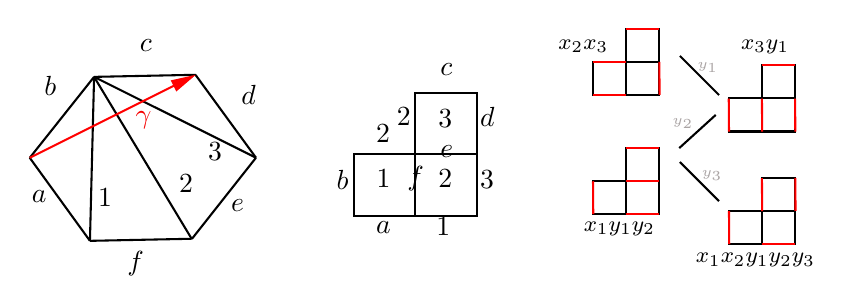
\begin{tikzpicture}[x=0.75pt,y=0.75pt,yscale=-1,xscale=1]
%uncomment if require: \path (0,437); %set diagram left start at 0, and has height of 437

%Straight Lines [id:da4908232703769615] 
\draw    (90.5,210) -- (119.5,250) ;
%Straight Lines [id:da17650145113834725] 
\draw    (90.5,210) -- (121.5,171) ;
%Straight Lines [id:da7174102064637746] 
\draw    (121.5,171) -- (170.5,170) ;
%Straight Lines [id:da8596665591342445] 
\draw    (119.5,250) -- (168.5,249) ;
%Straight Lines [id:da6279303631093601] 
\draw    (199.5,209.95) -- (170.37,170.04) ;
%Straight Lines [id:da7242109050720578] 
\draw    (199.5,209.95) -- (168.63,249.05) ;
%Straight Lines [id:da03863244955219047] 
\draw    (121.5,171) -- (119.5,250) ;
%Straight Lines [id:da31854017369699694] 
\draw    (121.5,171) -- (168.5,249) ;
%Straight Lines [id:da47134283434636637] 
\draw    (121.5,171) -- (199.5,209.95) ;
%Straight Lines [id:da5992871763576858] 
\draw [color={rgb, 255:red, 255; green, 0; blue, 0 }  ,draw opacity=1 ]   (90.5,210) -- (168.71,170.89) ;
\draw [shift={(170.5,170)}, rotate = 153.43] [fill={rgb, 255:red, 255; green, 0; blue, 0 }  ,fill opacity=1 ][line width=0.08]  [draw opacity=0] (12,-3) -- (0,0) -- (12,3) -- cycle    ;
%Shape: Square [id:dp11810124584691684] 
\draw   (246.63,208.3) -- (276.33,208.3) -- (276.33,238) -- (246.63,238) -- cycle ;
%Shape: Square [id:dp13699116965413383] 
\draw   (276.33,208.3) -- (306.03,208.3) -- (306.03,238) -- (276.33,238) -- cycle ;
%Shape: Square [id:dp1790172677132683] 
\draw   (276.33,178.6) -- (306.03,178.6) -- (306.03,208.3) -- (276.33,208.3) -- cycle ;
%Shape: Square [id:dp2883938512500389] 
\draw   (361.88,163.78) -- (377.86,163.78) -- (377.86,179.75) -- (361.88,179.75) -- cycle ;
%Shape: Square [id:dp7088947878360049] 
\draw   (377.86,163.78) -- (393.84,163.78) -- (393.84,179.75) -- (377.86,179.75) -- cycle ;
%Shape: Square [id:dp3954910092087409] 
\draw   (377.86,147.8) -- (393.84,147.8) -- (393.84,163.78) -- (377.86,163.78) -- cycle ;
%Shape: Rectangle [id:dp179337128236425] 
\draw   (427.39,181.35) -- (443.37,181.35) -- (443.37,197.33) -- (427.39,197.33) -- cycle ;
%Shape: Rectangle [id:dp839678338902704] 
\draw   (443.37,181.35) -- (459.34,181.35) -- (459.34,197.33) -- (443.37,197.33) -- cycle ;
%Shape: Square [id:dp03950570157166866] 
\draw   (443.37,165.37) -- (459.34,165.37) -- (459.34,181.35) -- (443.37,181.35) -- cycle ;
%Shape: Square [id:dp6368269407485009] 
\draw   (361.88,221.29) -- (377.86,221.29) -- (377.86,237.27) -- (361.88,237.27) -- cycle ;
%Shape: Square [id:dp5080247361620098] 
\draw   (377.86,221.29) -- (393.84,221.29) -- (393.84,237.27) -- (377.86,237.27) -- cycle ;
%Shape: Square [id:dp3148822004848474] 
\draw   (377.86,205.32) -- (393.84,205.32) -- (393.84,221.29) -- (377.86,221.29) -- cycle ;
%Shape: Rectangle [id:dp447116954358052] 
\draw   (427.39,235.67) -- (443.37,235.67) -- (443.37,251.65) -- (427.39,251.65) -- cycle ;
%Shape: Square [id:dp4061650684840712] 
\draw   (443.37,235.67) -- (459.34,235.67) -- (459.34,251.65) -- (443.37,251.65) -- cycle ;
%Shape: Square [id:dp7947789399156008] 
\draw   (443.37,219.7) -- (459.34,219.7) -- (459.34,235.67) -- (443.37,235.67) -- cycle ;
%Straight Lines [id:da8786639629522955] 
\draw    (403.74,160.9) -- (422.6,179.75) ;
%Straight Lines [id:da09557684843452541] 
\draw    (403.74,212.03) -- (422.6,230.88) ;
%Straight Lines [id:da7301540036749984] 
\draw    (421,189.34) -- (403.42,205.32) ;
%Straight Lines [id:da9619766876540269] 
\draw [color={rgb, 255:red, 255; green, 0; blue, 0 }  ,draw opacity=1 ]   (361.88,163.78) -- (377.86,163.78) ;
%Straight Lines [id:da6633598084478148] 
\draw [color={rgb, 255:red, 255; green, 0; blue, 0 }  ,draw opacity=1 ]   (361.88,179.75) -- (377.86,179.75) ;
%Straight Lines [id:da867888427891212] 
\draw [color={rgb, 255:red, 255; green, 0; blue, 0 }  ,draw opacity=1 ]   (377.86,147.8) -- (393.84,147.8) ;
%Straight Lines [id:da591102205651237] 
\draw [color={rgb, 255:red, 255; green, 0; blue, 0 }  ,draw opacity=1 ]   (443.37,165.37) -- (459.34,165.37) ;
%Straight Lines [id:da6749513848128621] 
\draw [color={rgb, 255:red, 255; green, 0; blue, 0 }  ,draw opacity=1 ]   (377.86,205.32) -- (393.84,205.32) ;
%Straight Lines [id:da7958887267913386] 
\draw [color={rgb, 255:red, 255; green, 0; blue, 0 }  ,draw opacity=1 ]   (377.86,221.29) -- (393.84,221.29) ;
%Straight Lines [id:da4580741088081952] 
\draw [color={rgb, 255:red, 255; green, 0; blue, 0 }  ,draw opacity=1 ]   (377.86,237.27) -- (393.84,237.27) ;
%Straight Lines [id:da08524721193125528] 
\draw [color={rgb, 255:red, 255; green, 0; blue, 0 }  ,draw opacity=1 ]   (443.37,251.65) -- (459.34,251.65) ;
%Straight Lines [id:da7449561570332422] 
\draw [color={rgb, 255:red, 255; green, 0; blue, 0 }  ,draw opacity=1 ]   (393.94,179.65) -- (393.84,163.78) ;
%Straight Lines [id:da7201215013298098] 
\draw [color={rgb, 255:red, 255; green, 0; blue, 0 }  ,draw opacity=1 ]   (361.99,237.16) -- (361.88,221.29) ;
%Straight Lines [id:da9147778038385569] 
\draw [color={rgb, 255:red, 255; green, 0; blue, 0 }  ,draw opacity=1 ]   (427.39,197.33) -- (427.28,181.46) ;
%Straight Lines [id:da1736214385948459] 
\draw [color={rgb, 255:red, 255; green, 0; blue, 0 }  ,draw opacity=1 ]   (443.37,197.33) -- (443.26,181.46) ;
%Straight Lines [id:da7301284550283822] 
\draw [color={rgb, 255:red, 255; green, 0; blue, 0 }  ,draw opacity=1 ]   (459.34,197.33) -- (459.24,181.46) ;
%Straight Lines [id:da8545909194796913] 
\draw [color={rgb, 255:red, 255; green, 0; blue, 0 }  ,draw opacity=1 ]   (443.37,235.67) -- (443.26,219.8) ;
%Straight Lines [id:da4475029716801513] 
\draw [color={rgb, 255:red, 255; green, 0; blue, 0 }  ,draw opacity=1 ]   (459.45,235.57) -- (459.34,219.7) ;
%Straight Lines [id:da433658880536243] 
\draw [color={rgb, 255:red, 255; green, 0; blue, 0 }  ,draw opacity=1 ]   (427.5,251.54) -- (427.39,235.67) ;


% Text Node
\draw (140,186.4) node [anchor=north west][inner sep=0.75pt]    {$\textcolor[rgb]{0.96,0,0}{\gamma }$};
% Text Node
\draw (90,224.4) node [anchor=north west][inner sep=0.75pt]    {$a$};
% Text Node
\draw (96,169.4) node [anchor=north west][inner sep=0.75pt]    {$b$};
% Text Node
\draw (142,151.4) node [anchor=north west][inner sep=0.75pt]    {$c$};
% Text Node
\draw (191,173.4) node [anchor=north west][inner sep=0.75pt]    {$d$};
% Text Node
\draw (186,228.4) node [anchor=north west][inner sep=0.75pt]    {$e$};
% Text Node
\draw (136,253.4) node [anchor=north west][inner sep=0.75pt]    {$f$};
% Text Node
\draw (122,223.4) node [anchor=north west][inner sep=0.75pt]    {$1$};
% Text Node
\draw (161,216.4) node [anchor=north west][inner sep=0.75pt]    {$2$};
% Text Node
\draw (175,201.4) node [anchor=north west][inner sep=0.75pt]    {$3$};
% Text Node
\draw (256.13,214.38) node [anchor=north west][inner sep=0.75pt]    {$1$};
% Text Node
\draw (285.88,214.38) node [anchor=north west][inner sep=0.75pt]    {$2$};
% Text Node
\draw (285.88,185.38) node [anchor=north west][inner sep=0.75pt]    {$3$};
% Text Node
\draw (236.88,214.38) node [anchor=north west][inner sep=0.75pt]    {$b$};
% Text Node
\draw (255.88,239.38) node [anchor=north west][inner sep=0.75pt]    {$a$};
% Text Node
\draw (255.88,192.38) node [anchor=north west][inner sep=0.75pt]    {$2$};
% Text Node
\draw (265.88,184.38) node [anchor=north west][inner sep=0.75pt]    {$2$};
% Text Node
\draw (270.88,212.38) node [anchor=north west][inner sep=0.75pt]    {$f$};
% Text Node
\draw (284.88,237.38) node [anchor=north west][inner sep=0.75pt]    {$1$};
% Text Node
\draw (286.88,202.38) node [anchor=north west][inner sep=0.75pt]    {$e$};
% Text Node
\draw (306.03,214.7) node [anchor=north west][inner sep=0.75pt]    {$3$};
% Text Node
\draw (306.03,184) node [anchor=north west][inner sep=0.75pt]    {$d$};
% Text Node
\draw (286.88,163.05) node [anchor=north west][inner sep=0.75pt]    {$c$};
% Text Node
\draw (343.75,151.65) node [anchor=north west][inner sep=0.75pt]  [font=\footnotesize]  {$x_{2} x_{3}$};
% Text Node
\draw (431.75,151.65) node [anchor=north west][inner sep=0.75pt]  [font=\footnotesize]  {$x_{3} y_{1}$};
% Text Node
\draw (355.99,239.56) node [anchor=north west][inner sep=0.75pt]  [font=\footnotesize]  {$x_{1} y_{1} y_{2}$};
% Text Node
\draw (409.99,254.56) node [anchor=north west][inner sep=0.75pt]  [font=\footnotesize]  {$x_{1} x_{2} y_{1} y_{2} y_{3}$};
% Text Node
\draw (410.65,162.45) node [anchor=north west][inner sep=0.75pt]  [font=\tiny,color={rgb, 255:red, 108; green, 98; blue, 98 }  ,opacity=0.58 ]  {$y_{1}$};
% Text Node
\draw (398.65,189.45) node [anchor=north west][inner sep=0.75pt]  [font=\tiny,color={rgb, 255:red, 108; green, 98; blue, 98 }  ,opacity=0.58 ]  {$y_{2}$};
% Text Node
\draw (412.65,214.45) node [anchor=north west][inner sep=0.75pt]  [font=\tiny,color={rgb, 255:red, 108; green, 98; blue, 98 }  ,opacity=0.58 ]  {$y_{3}$};


\end{tikzpicture}

\caption{In this figure we have a triangulated hexagon and an arc $\gamma$ (left), with its corresponding labeled snake graph $\s_{\gamma}$(center); and its perfect matchings with their corresponding monomials calculated through the expansion formula \ref{ExpansionFormula}.}
\end{figure}

To better explain how the height monomial works, we can see in the above figure that from the top left perfect matching (the one with only boundary edges, $P_-$) to the top right one, we are rotating tile 1, which gives the $y_1$ term. To then go to the bottom left, we rotate tile 2, which yields the term $y_2$. Finally, to go from bottom left to bottom right (the one with only boundary edges, $P_+$), we rotate tile 3 which yields the $y_3$ term. Moreover, the weight is calculated by looking at which edges are contained in the perfect matching. For example, in the top left perfect matching, we see that it contains edge 2 and 3 of our triangulation; these yield the $x_2$ and $x_3$ terms.

Finally, from Figure 2.7, we obtain that
\begin{equation*}
    x_{\gamma} = \dfrac{x_2x_3 + x_3y_1 + x_1y_1y_2 + x_1x_2y_1y_2y_3}{x_1x_2x_3}.
\end{equation*}

In the case of triangulated polygons, it is clear that there are finitely many arcs, up to isotopy; whilst in the case of, for example, an annulus, there are infinitely many arcs; e.g. we can have a curve that loops around the inner boundary component $n$ times. This is precisely why their corresponding Cluster algebras are finite and infinite, respectively. 

\section{Skein relations}
Suppose we have two arcs $\gamma_1,\gamma_2$ such that they intersect at some point $x$. Then we can define a concept called \emph{smoothing at $x$}; which is a collection of pairs $\{\gamma_3,\gamma_4\}$ and $\{\gamma_5,\gamma_6\}$ obtained from $\{\gamma_1,\gamma_2\}$ by replacing the crossing \KPB; in a small neighborhood of $x$, with the pair \KPC and \KPD. 
\begin{figure}[H]
    \centering


\tikzset{every picture/.style={line width=0.75pt}} %set default line width to 0.75pt        

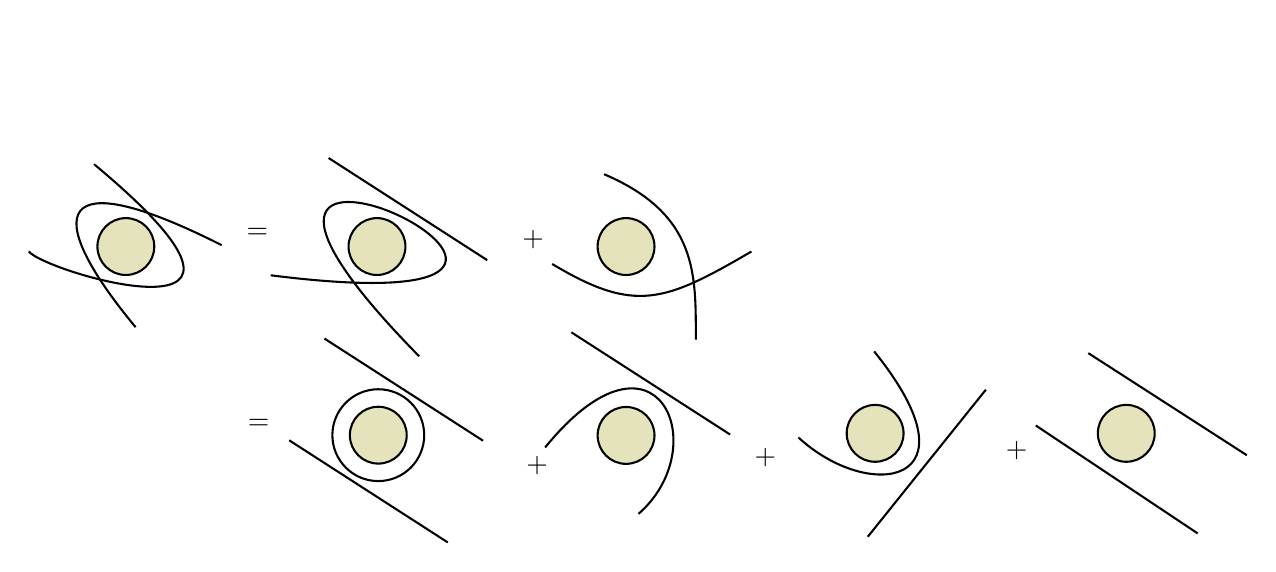
\begin{tikzpicture}[x=0.75pt,y=0.75pt,yscale=-1,xscale=1]
%uncomment if require: \path (0,300); %set diagram left start at 0, and has height of 300

%Shape: Circle [id:dp7164727092292058] 
\draw  [fill={rgb, 255:red, 228; green, 227; blue, 188 }  ,fill opacity=1 ] (63,133.8) .. controls (63,126.23) and (69.13,120.1) .. (76.7,120.1) .. controls (84.27,120.1) and (90.4,126.23) .. (90.4,133.8) .. controls (90.4,141.37) and (84.27,147.5) .. (76.7,147.5) .. controls (69.13,147.5) and (63,141.37) .. (63,133.8) -- cycle ;
%Curve Lines [id:da4188364150873798] 
\draw    (29.9,136.15) .. controls (38.4,146.65) and (170.9,185.15) .. (61.4,94.15) ;
%Curve Lines [id:da7397926385822463] 
\draw    (81.4,172.65) .. controls (35.4,117.15) and (42.2,92.35) .. (122.9,133.15) ;
%Straight Lines [id:da5533429251019936] 
\draw    (174.4,91.15) -- (250.8,140.35) ;
%Curve Lines [id:da9637986309064092] 
\draw    (146.5,147.65) .. controls (369.1,175.8) and (62.8,28.85) .. (218,186.65) ;
%Curve Lines [id:da5730466699163983] 
\draw    (307.1,98.95) .. controls (352.52,118.28) and (351.3,147.6) .. (351.3,178.6) ;
%Curve Lines [id:da377050407824876] 
\draw    (282.1,142.2) .. controls (322.1,166.2) and (336.3,160.54) .. (378.1,136.2) ;
%Straight Lines [id:da4567118907128783] 
\draw    (172.4,178.15) -- (248.8,227.35) ;
%Straight Lines [id:da9944916425980186] 
\draw    (155.4,227.15) -- (231.8,276.35) ;
%Shape: Circle [id:dp4153786288701671] 
\draw   (176.2,224.68) .. controls (176.2,212.46) and (186.11,202.55) .. (198.32,202.55) .. controls (210.54,202.55) and (220.45,212.46) .. (220.45,224.68) .. controls (220.45,236.89) and (210.54,246.8) .. (198.32,246.8) .. controls (186.11,246.8) and (176.2,236.89) .. (176.2,224.68) -- cycle ;
%Curve Lines [id:da007991355624611951] 
\draw    (278.7,230.6) .. controls (332.7,164.3) and (360.7,230.3) .. (323.7,262.6) ;
%Straight Lines [id:da05879559895469377] 
\draw    (291.4,175.15) -- (367.8,224.35) ;
%Curve Lines [id:da694044951364646] 
\draw    (437.24,184.34) .. controls (489.7,249.3) and (434.7,257.3) .. (400.72,225.76) ;
%Straight Lines [id:da6309735851468482] 
\draw    (491.06,202.76) -- (434.16,273.61) ;
%Straight Lines [id:da32536832233258217] 
\draw    (515.1,220) -- (593.1,272) ;
%Straight Lines [id:da04214537825490794] 
\draw    (540.4,185.15) -- (616.8,234.35) ;
%Shape: Circle [id:dp055172114017479124] 
\draw  [fill={rgb, 255:red, 228; green, 227; blue, 188 }  ,fill opacity=1 ] (184,133.8) .. controls (184,126.23) and (190.13,120.1) .. (197.7,120.1) .. controls (205.27,120.1) and (211.4,126.23) .. (211.4,133.8) .. controls (211.4,141.37) and (205.27,147.5) .. (197.7,147.5) .. controls (190.13,147.5) and (184,141.37) .. (184,133.8) -- cycle ;
%Shape: Circle [id:dp06546394326732974] 
\draw  [fill={rgb, 255:red, 228; green, 227; blue, 188 }  ,fill opacity=1 ] (304,133.8) .. controls (304,126.23) and (310.13,120.1) .. (317.7,120.1) .. controls (325.27,120.1) and (331.4,126.23) .. (331.4,133.8) .. controls (331.4,141.37) and (325.27,147.5) .. (317.7,147.5) .. controls (310.13,147.5) and (304,141.37) .. (304,133.8) -- cycle ;
%Shape: Circle [id:dp10396248031580357] 
\draw  [fill={rgb, 255:red, 228; green, 227; blue, 188 }  ,fill opacity=1 ] (184.63,224.68) .. controls (184.63,217.11) and (190.76,210.98) .. (198.32,210.98) .. controls (205.89,210.98) and (212.02,217.11) .. (212.02,224.68) .. controls (212.02,232.24) and (205.89,238.37) .. (198.32,238.37) .. controls (190.76,238.37) and (184.63,232.24) .. (184.63,224.68) -- cycle ;
%Shape: Circle [id:dp10282109383153959] 
\draw  [fill={rgb, 255:red, 228; green, 227; blue, 188 }  ,fill opacity=1 ] (304,224.8) .. controls (304,217.23) and (310.13,211.1) .. (317.7,211.1) .. controls (325.27,211.1) and (331.4,217.23) .. (331.4,224.8) .. controls (331.4,232.37) and (325.27,238.5) .. (317.7,238.5) .. controls (310.13,238.5) and (304,232.37) .. (304,224.8) -- cycle ;
%Shape: Circle [id:dp6810690428961315] 
\draw  [fill={rgb, 255:red, 228; green, 227; blue, 188 }  ,fill opacity=1 ] (424,223.8) .. controls (424,216.23) and (430.13,210.1) .. (437.7,210.1) .. controls (445.27,210.1) and (451.4,216.23) .. (451.4,223.8) .. controls (451.4,231.37) and (445.27,237.5) .. (437.7,237.5) .. controls (430.13,237.5) and (424,231.37) .. (424,223.8) -- cycle ;
%Shape: Circle [id:dp8686972692006888] 
\draw  [fill={rgb, 255:red, 228; green, 227; blue, 188 }  ,fill opacity=1 ] (545,223.8) .. controls (545,216.23) and (551.13,210.1) .. (558.7,210.1) .. controls (566.27,210.1) and (572.4,216.23) .. (572.4,223.8) .. controls (572.4,231.37) and (566.27,237.5) .. (558.7,237.5) .. controls (551.13,237.5) and (545,231.37) .. (545,223.8) -- cycle ;

% Text Node
\draw (133.4,123.75) node [anchor=north west][inner sep=0.75pt]    {$=$};
% Text Node
\draw (266.2,124.4) node [anchor=north west][inner sep=0.75pt]    {$+$};
% Text Node
\draw (134,215.4) node [anchor=north west][inner sep=0.75pt]    {$=$};
% Text Node
\draw (268.2,233.4) node [anchor=north west][inner sep=0.75pt]    {$+$};
% Text Node
\draw (378.2,229.4) node [anchor=north west][inner sep=0.75pt]    {$+$};
% Text Node
\draw (499.2,226.4) node [anchor=north west][inner sep=0.75pt]    {$+$};


\end{tikzpicture}


\caption{Example of a smoothing process.}
\end{figure}
In \cite{MW}, the authors proved the following; also known as the \emph{Skein relations};
\begin{theorem}[Skein relations]\label{Skeinrelations}
    If $\{\gamma_3,\gamma_4\}$ and $\{\gamma_5,\gamma_6\}$ are curves obtained from $\{\gamma_1,\gamma_2\}$ through a smoothing process, then 
    \begin{equation*}
        x_{\gamma_1}x_{\gamma_2} = y_{34}x_{\gamma_3}x_{\gamma_4} + y_{56}x_{\gamma_5}x_{\gamma_6};
    \end{equation*}
    for some $y_{34},y_{56}$ in $\mathcal{G}$ and $x_{\gamma_i}$ is the cluster algebra element corresponding to the arc $\gamma_i$. Moreover, we  if we apply this to a self-crossing curve $\gamma$, through which we obtain $\gamma_1$ and $\gamma_2$, then
    \begin{equation*}
        x_{\gamma} = y_1x_{\gamma_1} + y_2x_{\gamma_2};
    \end{equation*}
    for some $y_1,y_2$ in $\mathcal{G}$. 
\end{theorem}
It turns out that, by using Skein relations, we find that a product of cluster variables corresponds to an arc in the surface. If we let $\mathcal{B}$ be the collection of all the curves that arise by applying the smoothing process to all possible curves, we get that $\mathcal{B}$ forms a basis for the cluster algebra $\mathcal{A} = \mathcal{A}(\mathbf{x},\mathbf{y},\mathcal{Q})$. This has been proven in \cite{MSW}.